% Бүлэг 1

\chapter{Системийн тухай онол, арга зүйн судалгаа} % Бүлгийн нэр
\label{Chapter1} % Энэ бүлэг рүү ишлэл хийх бол \ref{Chapter1} командыг ашигла 

%-------------------------------------------------------------------------------

% Агуулгад ашигласан хэвшүүлэлтийн зарим командын тодорхойлолт
\newcommand{\keyword}[1]{\textbf{#1}}
\newcommand{\tabhead}[1]{\textbf{#1}}
\newcommand{\code}[1]{\texttt{#1}}
\newcommand{\file}[1]{\texttt{\bfseries#1}}
\newcommand{\option}[1]{\texttt{\itshape#1}}

%-------------------------------------------------------------------------------



%-------------------------------------------------------------------------------
\section{Ажлын байрны сонгон шалгаруулалтын тухай}
\par{}
Ажилд авах үйл явц нь байгууллагын хүний нөөцийн хамгийн чухал үйл ажиллагааны нэг бөгөөд зөв ажилтныг зөв албан тушаалд сонгох шийдвэрээс байгууллагын бүтээмж, өрсөлдөх чадвар шууд хамаардаг.

Уламжлалт ажилд авах процесс нь дараах үндсэн үе шатуудаас бүрдэнэ:
\begin{itemize}
    \item Ажлын байрны шаардлага тодорхойлох;
    \item Ажил горилогчдыг татах;
    \item CV болон анкет хүлээн авах;
    \item Урьдчилсан шүүлт хийх;
    \item Ярилцлага болон үнэлгээ;
    \item Эцсийн сонголт хийх.
\end{itemize}

\par{}Гэвч энэхүү процесс нь ихэвчлэн гараар хийгддэг бөгөөд их хэмжээний мэдээлэл боловсруулах шаардлагатай байдаг. Нэг ажлын байрны хувьд олон зуун CV ирдэг тул хүний нөөцийн ажилтнуудын хувьд бүх мэдээллийг үнэн зөв, хурдан боловсруулахад хүндрэлтэй байдаг.

Үүний улмаас дараах асуудлууд үүсдэг:
\begin{itemize}
    \item Цаг хугацаа их зарцуулдаг;
    \item Хүний субъектив алдаа гардаг;
    \item Зарим тохиромжтой ажил горилогчийг алдах магадлалтай.
\end{itemize}
Иймээс ажилд авах процессыг автоматжуулах, өгөгдөлд суурилсан шийдвэр гаргах шаардлага бий болсон.
\section{Уламжлалт болон AI-д суурилсан сонгон шалгаруулалт}

\par{}Уламжлалт ажилд авах арга нь ихэвчлэн хүний оролцоонд тулгуурласан, гараар гүйцэтгэдэг процесс байдаг. Хүний нөөцийн ажилтнууд CV-үүдийг нэг бүрчлэн уншиж, шаардлагад нийцэж байгаа эсэхийг субъектив байдлаар үнэлдэг. Энэ арга нь ойлгомжтой, хэрэгжүүлэхэд хялбар боловч дараах сул талуудтай:

\begin{itemize}
    \item Их хэмжээний цаг хугацаа шаарддаг;
    \item Хүний субъектив үнэлгээ их нөлөөлдөг;
    \item Олон ажил горилогчтой үед үр ашиг буурдаг;
    \item Зарим тохиромжтой ажил горилогчийг алдах магадлалтай.
\end{itemize}   

\par{}Орчин үед хиймэл оюун ухаанд (AI) суурилсан ажилд авах системүүд өргөн хэрэглэгдэж эхэлсэн. Эдгээр системүүд нь машин сургалт (ML) болон байгалийн хэл боловсруулалт (NLP)-ын аргуудыг ашиглан CV болон ажлын байрны тодорхойлолтыг автоматаар боловсруулж, ажил горилогчийн тохирлыг үнэлдэг.

AI-д суурилсан системүүдийн давуу талууд:
\begin{itemize}
    \item Том хэмжээний өгөгдлийг хурдан боловсруулах чадвартай;
    \item Шийдвэр гаргалтыг өгөгдөлд суурилсан болгодог;
    \item Хүний алдаа болон bias-ыг багасгах боломжтой;
    \item Сонгон шалгаруулалтын хугацааг богиносгодог.
\end{itemize} 

\par{}Судалгаануудын үр дүнгээс харахад AI нь ажилд авах процессыг илүү үр ашигтай болгож, шийдвэр гаргалтын чанарыг сайжруулдаг\cite{smart_hiring_ai}.

Гэсэн хэдий ч AI системүүд нь зарим сул талтай. Үүнд:
\begin{itemize}
    \item Алгоритмын bias үүсэх эрсдэл;
    \item Өгөгдлийн нууцлалын асуудал;
    \item Системийн шийдвэрийг тайлбарлах хүндрэл.
\end{itemize}

\par{}Иймээс орчин үеийн судалгаанд зөвхөн AI ашиглах бус, тайлбарлах боломжтой (Explainable AI) систем хөгжүүлэх шаардлага чухал гэж үзэж байна.

%-------------------------------------------------------------------------------
\section{AI-д суурилсан үнэлгээний алгоритмууд}

\par{}Орчин үеийн ажилд авах системүүд нь хиймэл оюун ухаан, машин сургалт болон байгалийн хэл боловсруулалтын аргуудыг ашиглан ажил горилогчийг автоматаар үнэлэх боломжийг олгодог.

\par{}Юуны өмнө, машин сургалт нь өгөгдлөөс хэв маяг (pattern) илрүүлж, тухайн өгөгдөлд тулгуурлан таамаглал хийх чадвартай. Ажилд авах системийн хувьд ML алгоритмууд нь өмнөх сонгон шалгаруулалтын өгөгдлийг ашиглан ажил горилогчийн тохирлыг үнэлэхэд ашиглагддаг. Жишээлбэл, ангиллын алгоритмууд нь CV-ийг “тохиромжтой” эсвэл “тохиромжгүй” гэж ангилах боломжтой \cite{smart_hiring_ai}.

\par{}Байгалийн хэл боловсруулалт нь текстэн өгөгдлийг ойлгож, боловсруулахад чиглэгдсэн технологи бөгөөд CV болон ажлын байрны тодорхойлолт зэрэг бүтэцгүй өгөгдлийг анализ хийхэд чухал үүрэгтэй. NLP-ийн тусламжтайгаар ур чадвар, боловсрол, ажлын туршлага зэрэг мэдээллийг текстээс автоматаар ялган авах боломжтой \cite{nlp_resume_parsing}.

Resume screening-ийн орчин үеийн системүүдэд дараах NLP аргууд өргөн хэрэглэгддэг:
\begin{itemize}
    \item Named Entity Recognition (NER) – ур чадвар, байгууллага, боловсрол зэрэг мэдээллийг ялгах;
    \item Part-of-Speech Tagging – үгийн үүргийг тодорхойлох;
    \item Text vectorization – текстийг тоон хэлбэрт шилжүүлэх \cite{mikolov2013word2vec}.
\end{itemize}

\par{}Эдгээр боловсруулалтын дараа текстэн өгөгдлийг машин сургалтын алгоритмуудад оруулах боломж бүрддэг. Тухайлбал, K-Nearest Neighbors (KNN), Support Vector Machine (SVM) зэрэг алгоритмуудыг ашиглан CV болон ажлын байрны тохирлыг үнэлэх боломжтой \cite{nlp_resume_parsing}.

\par{}Сүүлийн үеийн судалгаанд deep learning болон embedding-д суурилсан аргууд илүү өргөн хэрэглэгдэж байна. Орчин үеийн томоохон хэлний загваруудын суурь болох Transformer архитектур \cite{vaswani2017attention} болон BERT зэрэг урьдчилан сургасан загварууд \cite{devlin2019bert} нь байгалийн хэлийг гүн гүнзгий ойлгох боломжийг нээсэн. Ялангуяа Sentence-BERT зэрэг pretrained language model-ууд нь текстийн утгын түвшний ижил төстэй байдлыг өндөр нарийвчлалтай тодорхойлох боломжийг олгодог \cite{reimers2019sentencebert}. Эдгээр аргууд нь CV болон ажлын байрны тодорхойлолтыг вектор орон зайд дүрслэн, cosine similarity ашиглан хоорондын нийцлийг тооцоолдог.

\par{}Мөн Siamese neural network архитектур нь хоёр текстийн хоорондын семантик хамаарлыг нэг ижил орон зайд сурч, илүү нарийвчлалтай matching хийх боломжийг бүрдүүлдэг \cite{resume_matching_siamese}.

Ерөнхийдөө AI алгоритмуудыг ашигласнаар:
\begin{itemize}
    \item CV screening процессыг автоматжуулах;
    \item Шийдвэр гаргалтыг илүү нарийвчлалтай болгох;
    \item Том хэмжээний өгөгдлийг хурдан боловсруулах.
\end{itemize}

\par{}Гэсэн хэдий ч эдгээр алгоритмууд нь ихэвчлэн “black-box” шинж чанартай байдаг тул гарсан үр дүнг тайлбарлахад хүндрэл үүсдэг. Иймээс AI системийн тайлбарлах чадварыг нэмэгдүүлэх нь чухал асуудал болж байна.
\subsection*{Алгоритмуудын товч тайлбар}

\par{}Support Vector Machine (SVM) нь ангиллын алгоритм бөгөөд өгөгдлийг хоёр ангилалд хамгийн сайн ялгах шулууныг (hyperplane) олох зарчимд тулгуурладаг. CV screening-д энэ алгоритм нь ажил горилогчийг “тохиромжтой” болон “тохиромжгүй” гэж ангилахад ашиглагдаж болно.

\par{}K-Nearest Neighbors (KNN) алгоритм нь шинэ өгөгдлийг өмнөх өгөгдлүүдтэй ойролцоогоор нь харьцуулж ангилдаг. Өөрөөр хэлбэл, хамгийн ойрхон K ширхэг хөрш өгөгдлийн ангилалд тулгуурлан шинэ өгөгдлийг тодорхойлдог.

\par{}Томоохон хэлний загвар (Large Language Model, LLM) нь гүн мэдрэлийн сүлжээнд суурилсан (deep neural network), байгалийн хэлийг гүн гүнзгий ойлгох чадвартай загвар юм \cite{brown2020gpt3}. LLM нь зөвхөн тоон ижил төстэй байдлыг тооцоолохоос гадна, CV болон ажлын шаардлагыг нарийн контекстийн хамт задлан шинжилж, тайлбартай үнэлгээ буцаах боломжтой. Энэхүү системд Anthropic компанийн Claude Sonnet LLM-ийг ашигласан \cite{anthropic2024claude}.

\par{}Энэхүү системийн чатбот нь PostgreSQL өгөгдлийн сангаас бүх идэвхтэй ажлын байрны мэдээллийг татаж, Claude-ийн prompt-д контекст болгон шууд дамжуулдаг. Ингэснээр LLM нь тухайн үеийн бодит ажлын байрны мэдээлэлд суурилан хэрэглэгчийн асуултад хариулт өгнө.

\section{Ижил төстэй системийн судалгаа}
\par{}Энэ хэсэгт ажлын байрны зар болон ажил горилогч ажилд орох болон ажилд авах үйл явц, мөн ажилд орох хүсэлт илгээсэн ажил олгогчдын чадварыг үнэлэх үйл ажиллагаатай холбоотой веб системүүдийн талаарх судалгааг хийсэн.
\par{} Манай улсад дээрх дурьдсан үйл явцтай холбоотой нэр бүхий системүүд бол \href{https://www.zangia.mn}{\textit{zangia.mn}} болон \href{https://lambda.global}{\textit{lambda.global}} юм. Эдгээр системүүдийн ялгааг доор харуулав.

\par{} \textbf{Zangia.mn:}
\par{}Zangia.mn нь Монголын хамгийн том ажлын зарын портал бөгөөд 2009 оноос хойш үйл ажиллагаагаа явуулж байгаа. Систем нь ажил горилогчид өөрийн мэдээллйиг оруулж, ажлын зар хайн, тухайн ажилд өөрийн нийцлийг шалгах боломжийг олгодог бол ажил олгогчид ажлын зарыг нийтлэх, ирсэн анкетуудыг удирдах боломжийг бүрдүүлдэг.

\par{}Zangia.mn системийн үндсэн боломжууд:
\begin{itemize}
    \item Ажлын зар нийтлэх, хайх болон шүүх;
    \item Өөрийн мэдээллийг оруулж, удирдах, CV гарган авах;
    \item Мобайл аппликейшн;
    \item Ажлын байрны мэдэгдэл (notification) илгээх;
    \item Өөрийн анкетийг тухайн ажлын байрны шаардлагад нийцэх эсэхийг шалгуулах.
\end{itemize}

\par{}Гэсэн хэдий ч Zangia.mn нь анкетыг хүлээн авснаас хойш ажил горилогчтой ярилцлага товлох гэх мэт ажил авах дараагийн шатны үйл ажиллагааг хамарсан функц байдаггүй. CV шүүлт болон ажил горилогчийн чадварын үнэлгээ нь хүний нөөцийн ажилтны гараар хийгддэг.

\par{}Зураг \ref{fig: z-ajliin-zar}-д систем рүү нэвтэрч орсны дараах нүүр хуудас буюу ажлын зар харах, шүүх хэсэг харагдаж байна.

\begin{figure}[H]
    \centering
    
\includegraphics[scale=0.3]{Figures/chapter1/zangia/ajliin_zar.png}
    \caption{Zangia.mn сайтын нүүр хуудас}
    \label{fig: z-ajliin-zar}
\end{figure}

\par{}Зураг \ref{fig: z-profile}-д системд оруулсан хэрэглэгчийн мэдээлэл харагдаж байгаа бөгөөд эдгээр мэдээллийг ашиглан өөрийн анкетыг гаргах авах хэсэг харагдаж байна.
\begin{figure}[H]
    \centering
    
\includegraphics[scale=0.3]{Figures/chapter1/zangia/profile.png}
    \caption{Zangia.mn сайтын профайлын хэсэг}
    \label{fig: z-profile}
\end{figure}

\par{}Зураг \ref{fig: z-result}-д сонгосон ажлын байр дээр өөрийн мэдээллийн дагуу тухайн ажилд тохирох эсэхийг шалгуулж, давуу болон сул талуудыг харьцуулж харуулсан байна.
\begin{figure}[H]
    \centering
    
\includegraphics[scale=0.3]{Figures/chapter1/zangia/result.png}
    \caption{Zangia.mn сайтын үнэлгээний хэсэг}
    \label{fig: z-result}
\end{figure}

\par{} \textbf{Lambda.global:}
\par{}Lambda.global нь мөн адил ажлын зарын сайт бөгөөд ажил горилогч болон ажил олгогчийг холбох платформ юм. Системийн гол онцлог нь мэргэжилтнүүдэд тохирсон ажлын зар, ажил горилогчдын ур чадварын мэдээллийг дэлгэрэнгүй оруулах боломжоор хангадаг явдал юм.

\par{}Lambda.global системийн үндсэн боломжууд:
\begin{itemize}
    \item Өөрийн анкетыг загварыг дагуу үүсгэх;
    \item Ур чадвар болон ажлын байраар хайх, шүүх;
    \item Ажил горилогчийн профайл болон портфолиог дэлгэрэнгүй байршуулах;
    \item Ажил олгогчид ажил горилогчийг урих боломж;
    \item Remote болон гадаадын ажлын байрны сонголтууд.
\end{itemize}

\par{}Lambda.global нь CV болон ажлын байрны хоорондох тохирлыг автоматаар тооцоолох, ажил горилогчийн ур чадварыг объектив байдлаар үнэлэх хиймэл оюун ухааны технологийг хэрэглэдэг ч гэсэн ажил горилогчтой ярилцлага товлох болон дараагийн шатны үйл явцыг агуулаагүй.

\par{}Зураг \ref{fig: l-ajliin-zar}-д систем рүү нэвтэрч орсны дараах нүүр хуудас буюу ажлын зар харах, шүүх хэсэг харагдаж байна.

\begin{figure}[H]
    \centering
    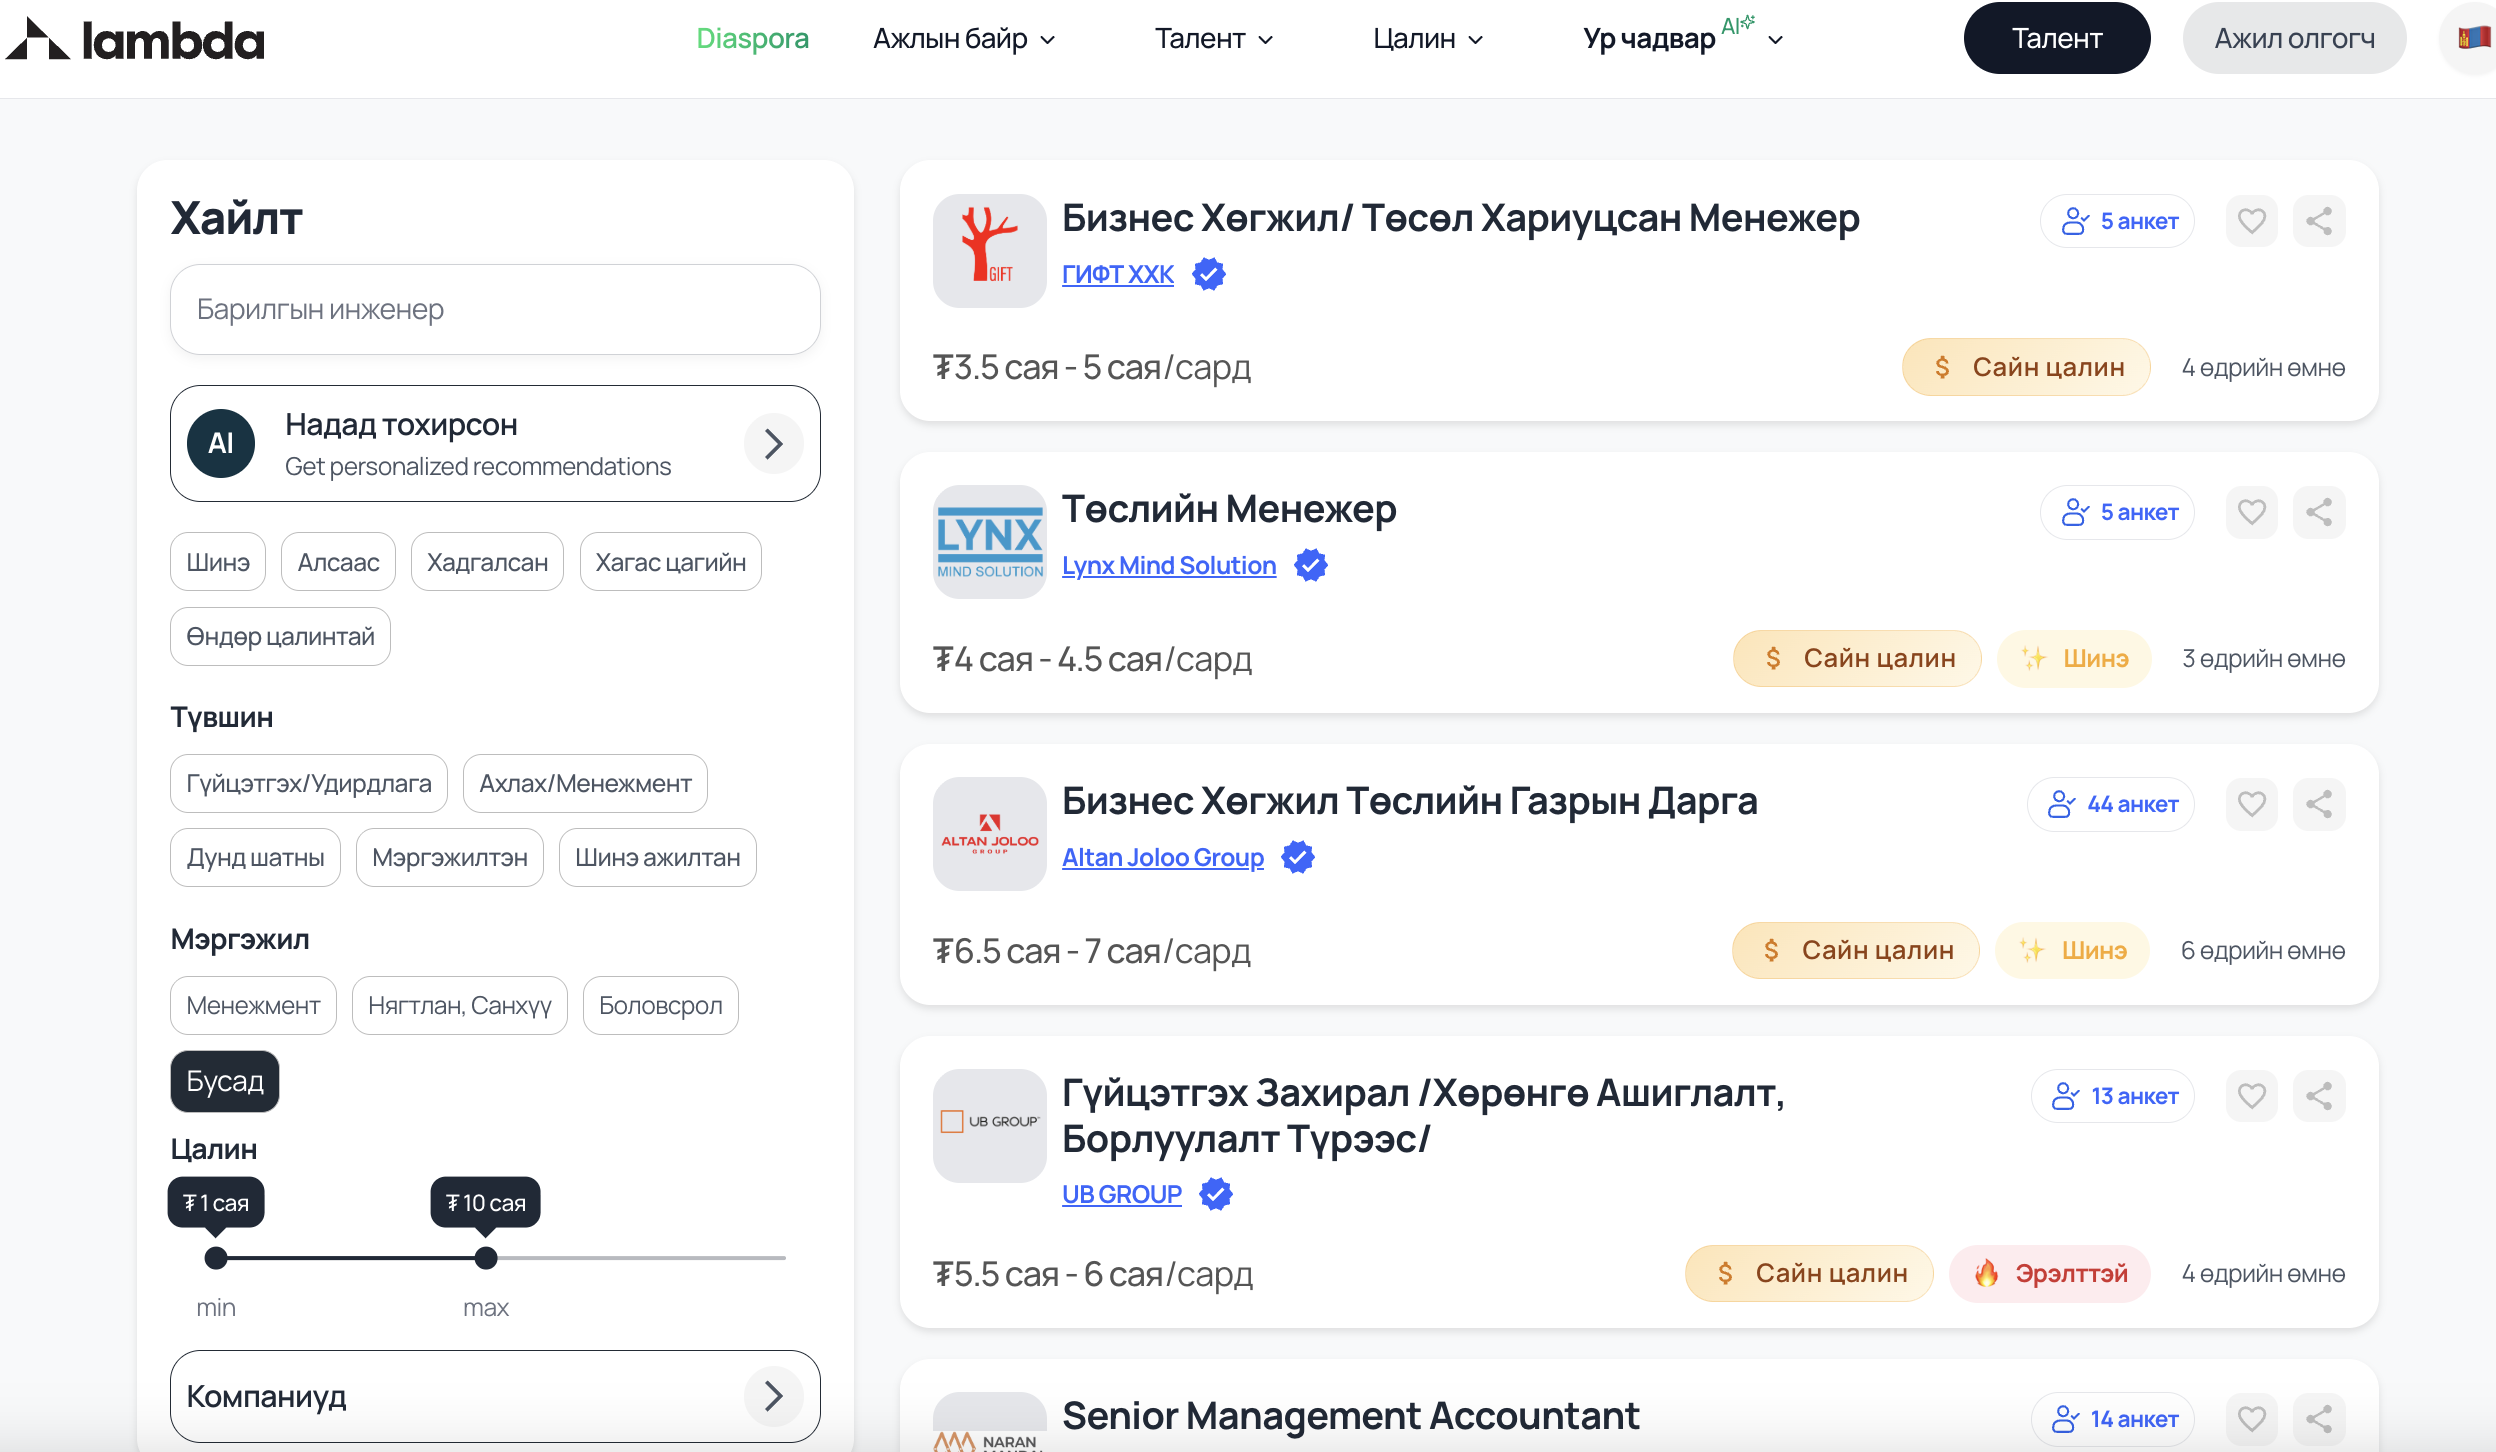
\includegraphics[scale=0.3]{Figures/chapter1/lambda/ajliin_zar.png}
    \caption{Zangia.mn сайтын нүүр хуудас}
    \label{fig: l-ajliin-zar}
\end{figure}

\par{}Зураг \ref{fig: l-profile}-д системд оруулсан хэрэглэгчийн мэдээлэл харагдаж байгаа бөгөөд эдгээр мэдээллийг ашиглан өөрийн анкетыг гаргах авах хэсэг харагдаж байна.
\begin{figure}[H]
    \centering
    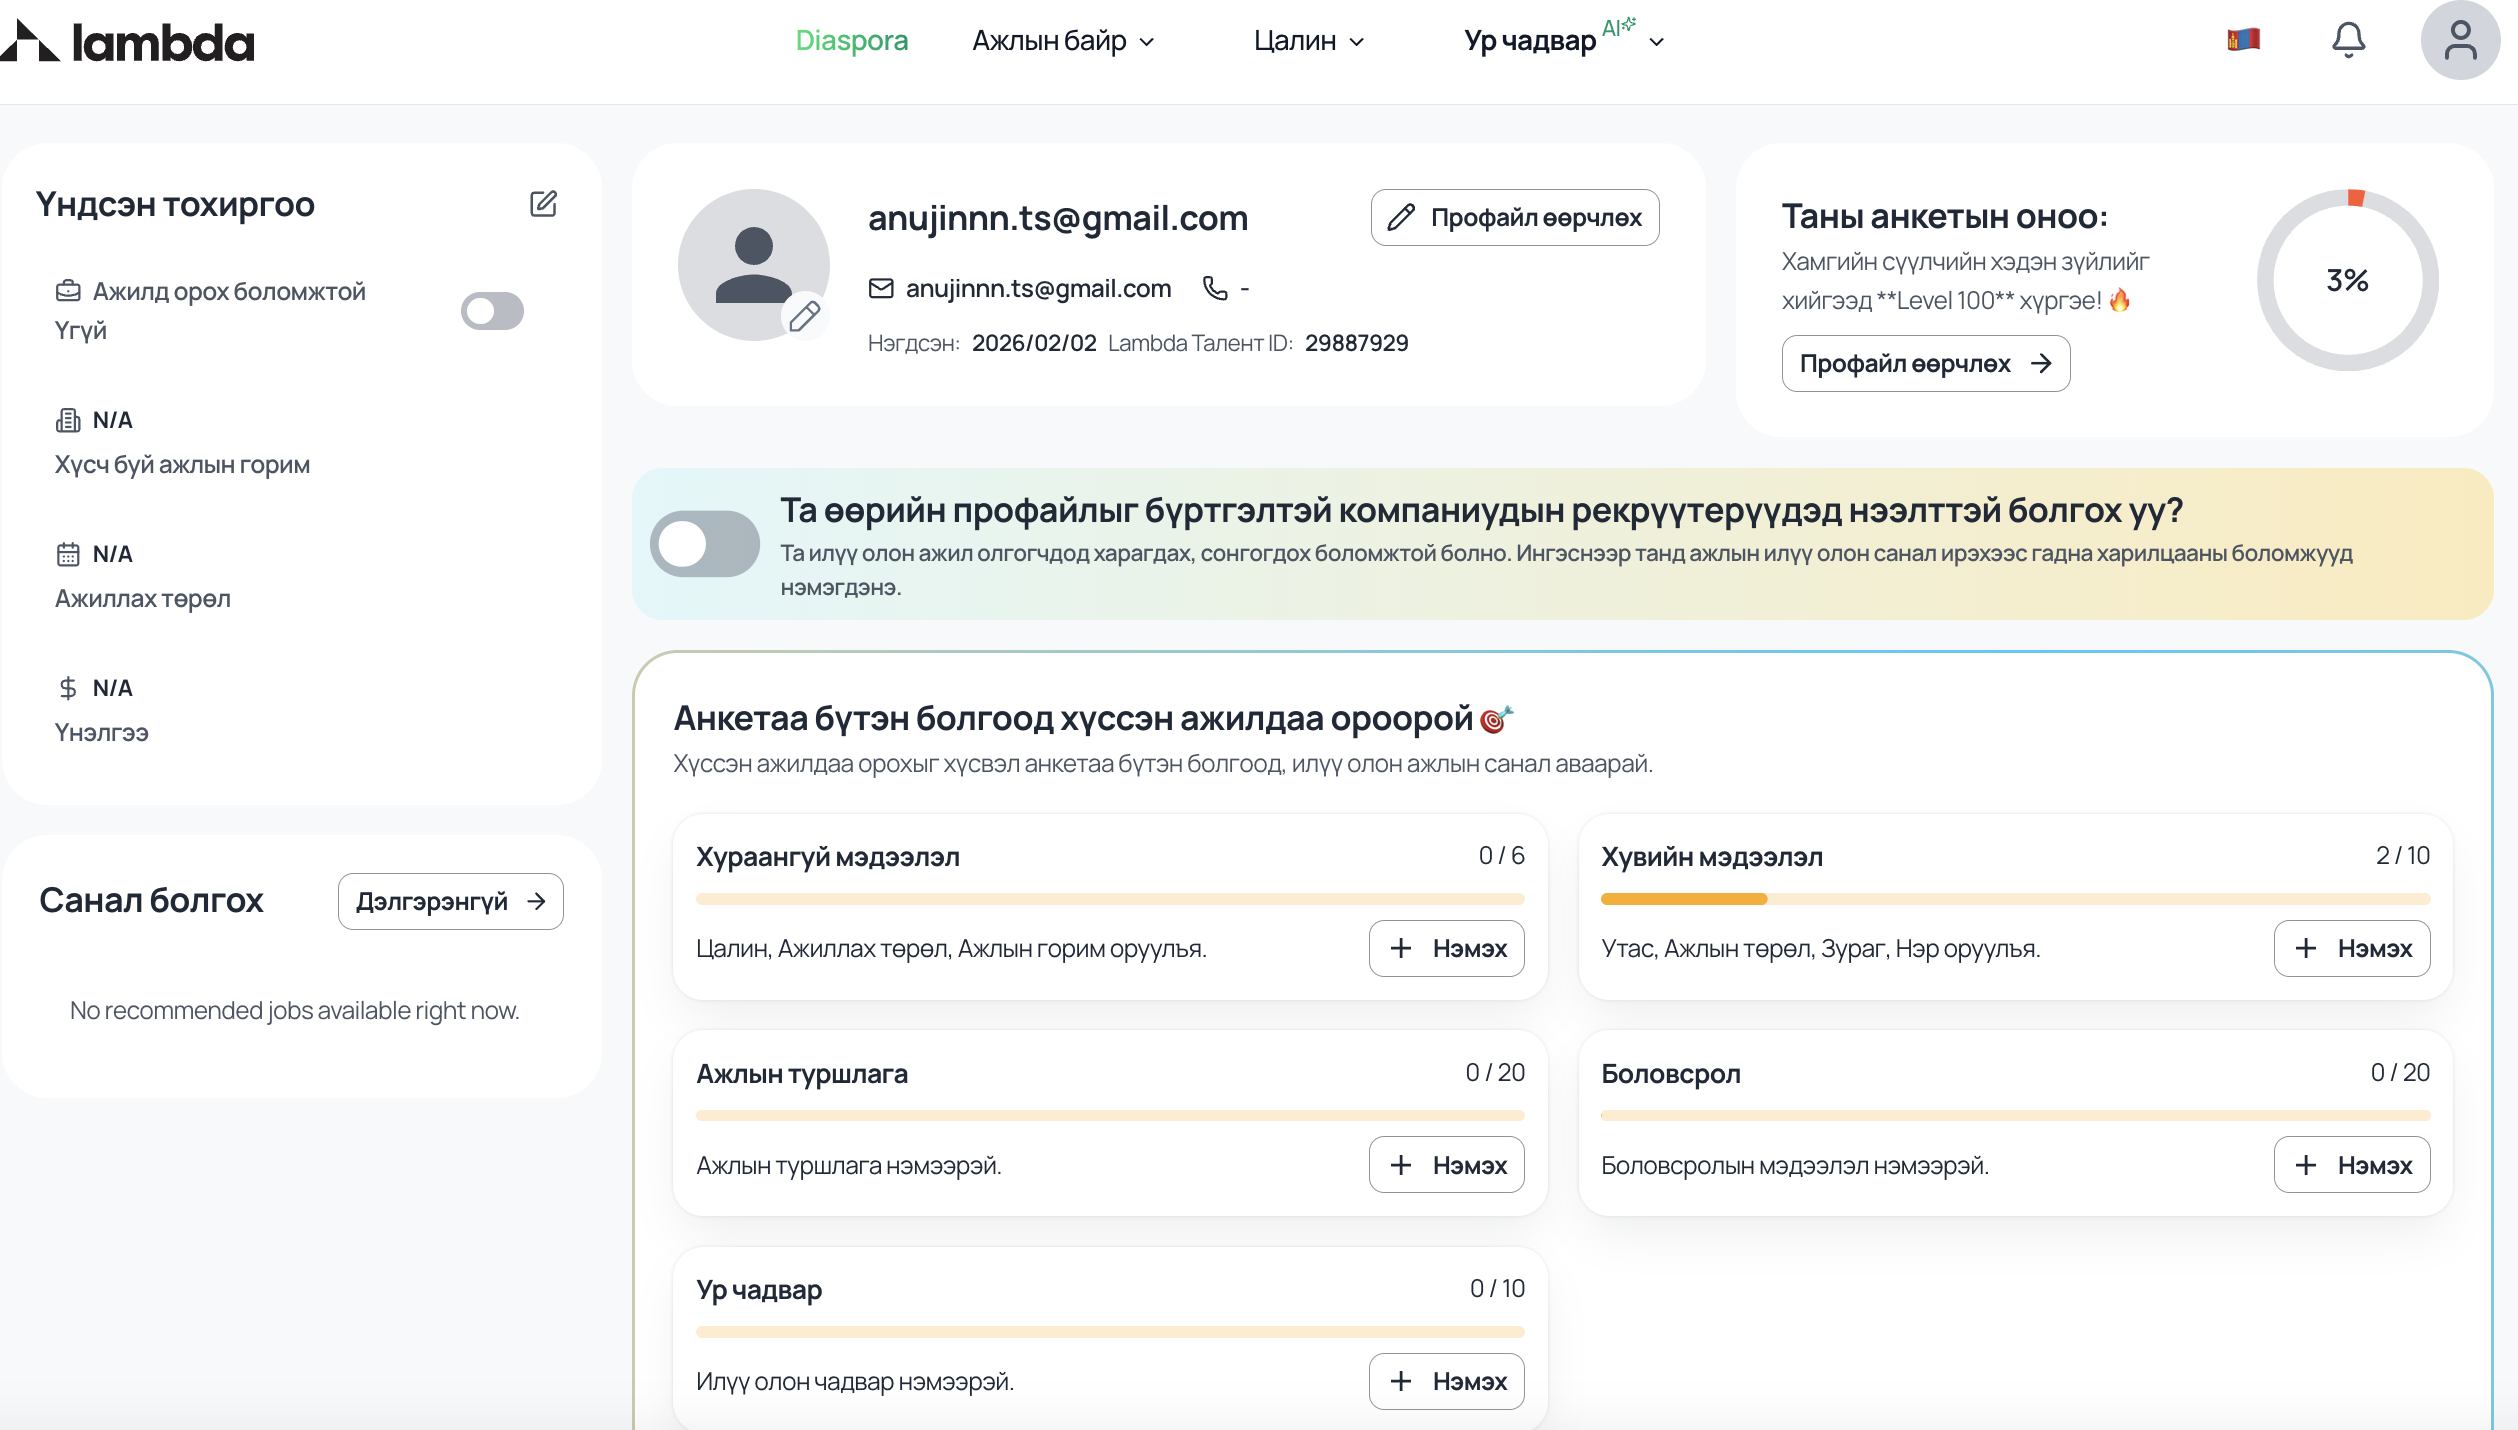
\includegraphics[scale=0.3]{Figures/chapter1/lambda/profile.png}
    \caption{Zangia.mn сайтын профайлын хэсэг}
    \label{fig: l-profile}
\end{figure}

\par{}Зураг \ref{fig: l-result}-д сонгосон ажлын байр дээр өөрийн мэдээллийн дагуу тухайн ажилд тохирох эсэхийг шалгуулах хэсэг харагдаж байна.
\begin{figure}[H]
    \centering
    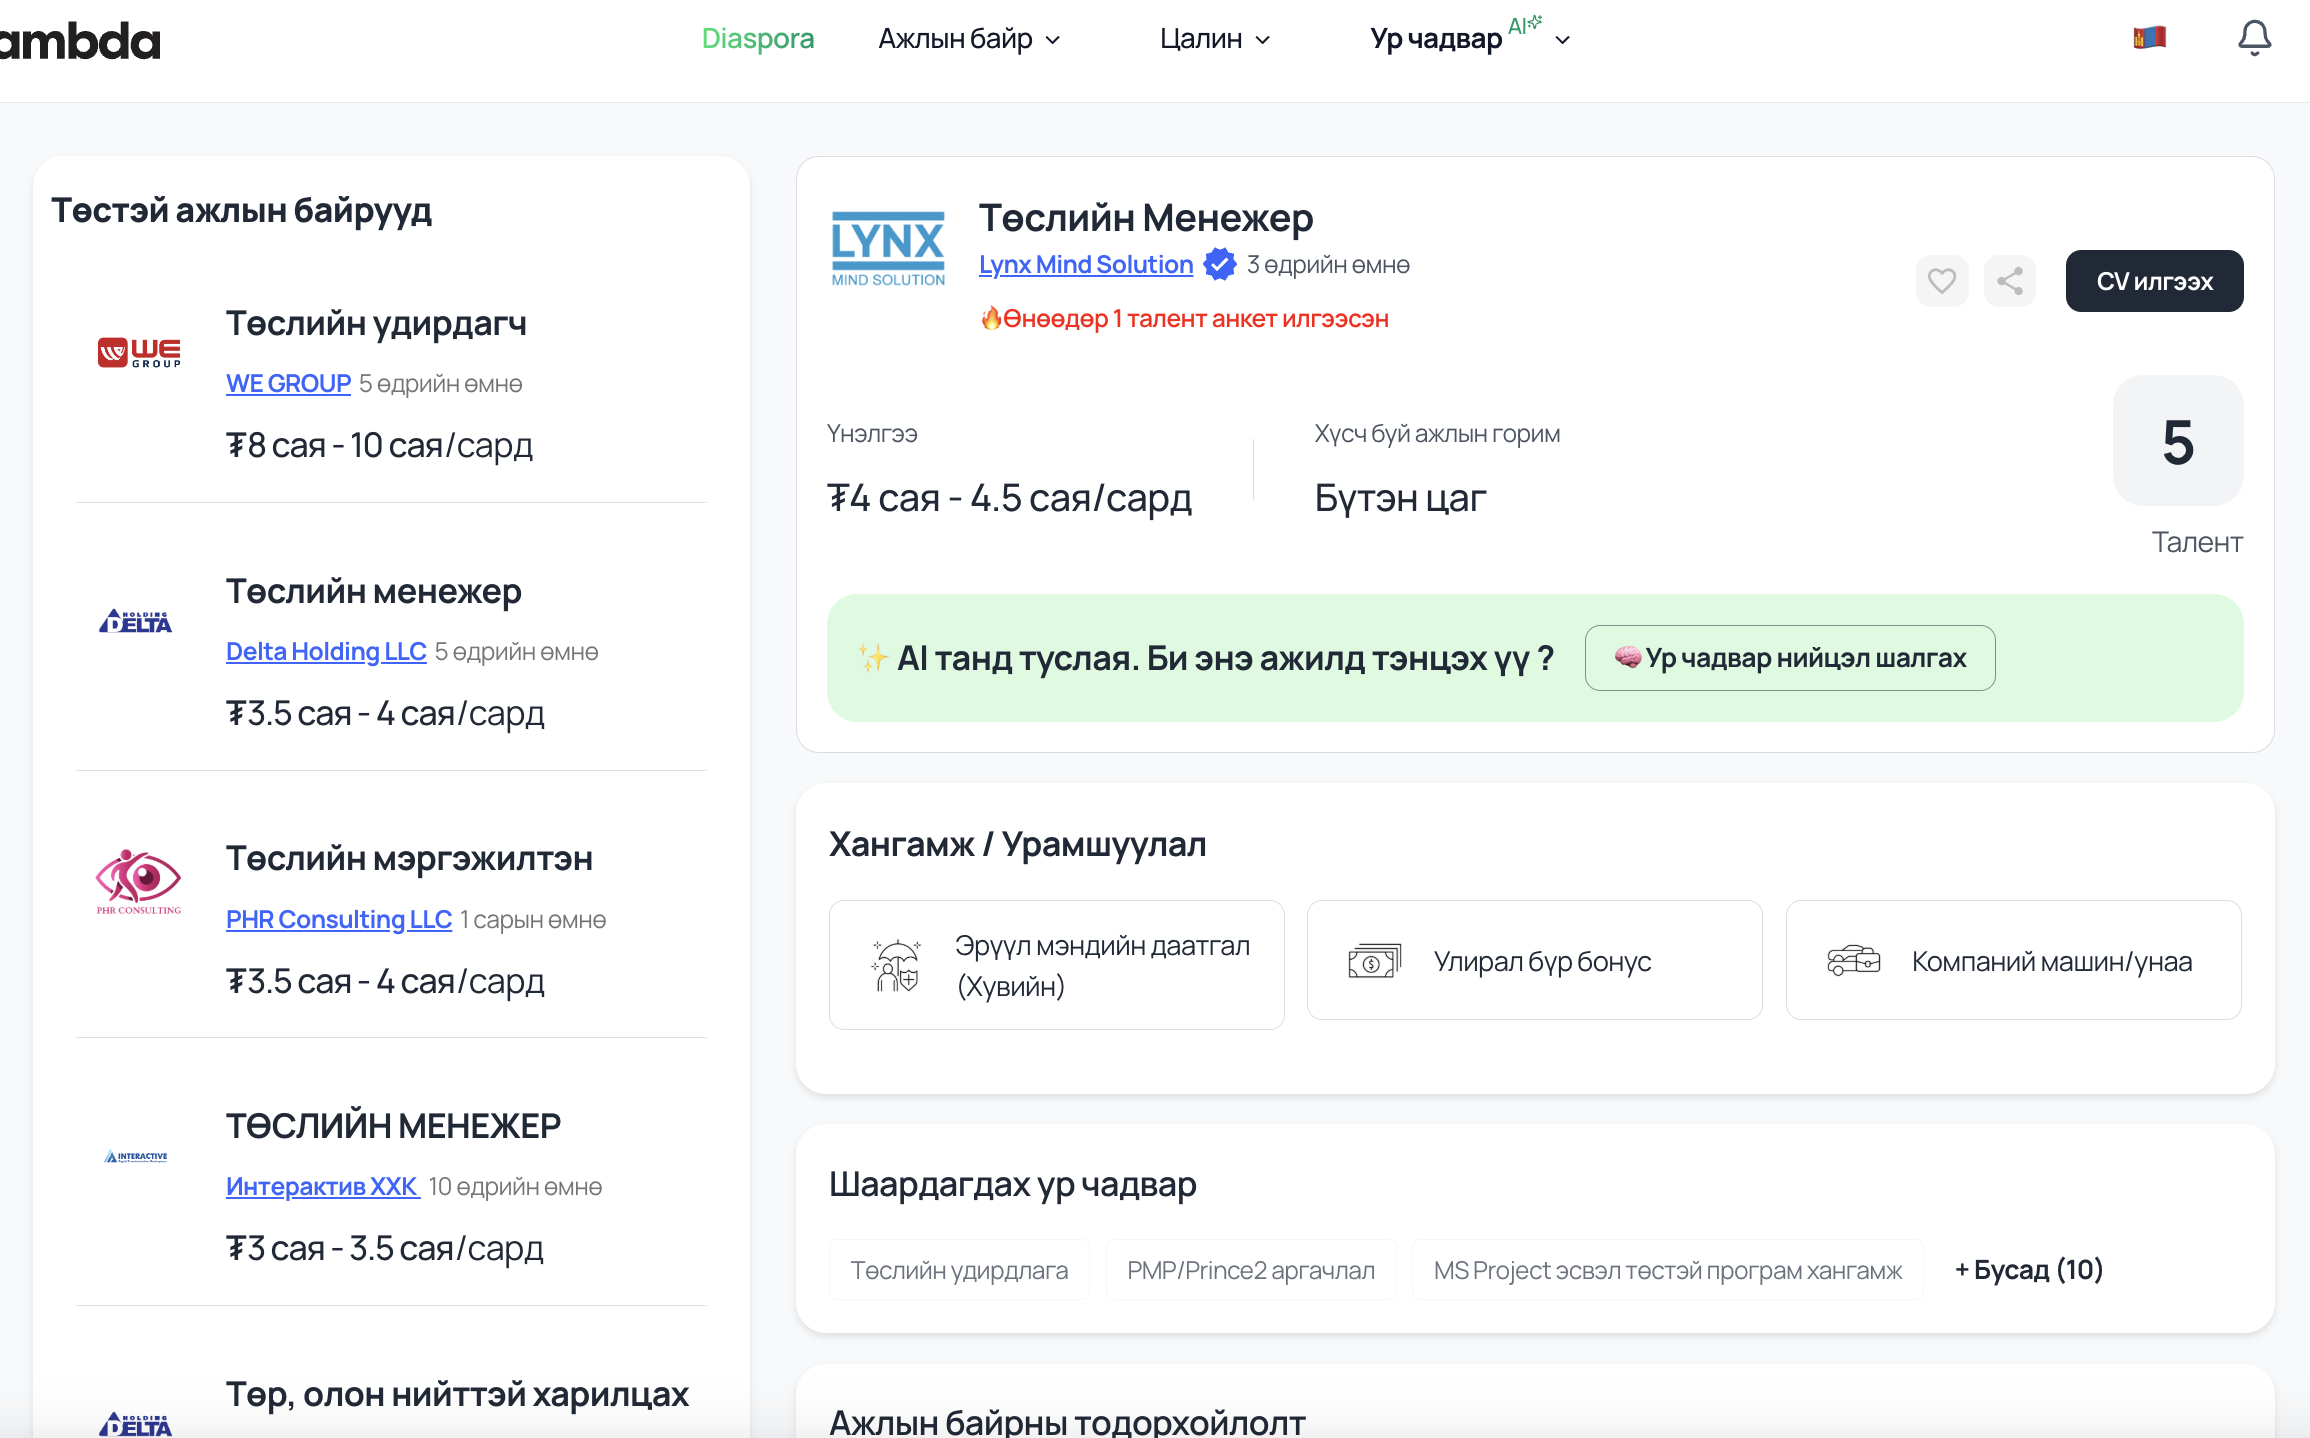
\includegraphics[scale=0.3]{Figures/chapter1/lambda/result.png}
    \caption{Zangia.mn сайтын үнэлгээний хэсэг}
    \label{fig: l-result}
\end{figure}

\par{}Зураг \ref{fig: l-cv}-д системд оруулсан өөрийн мэдээлэл болон намтарыг оруулснаар, тодорхой загварын дагуу өөрийн анкетыг үүсгэх, засах хэсэг харагдаж байна.
\begin{figure}[H]
    \centering
    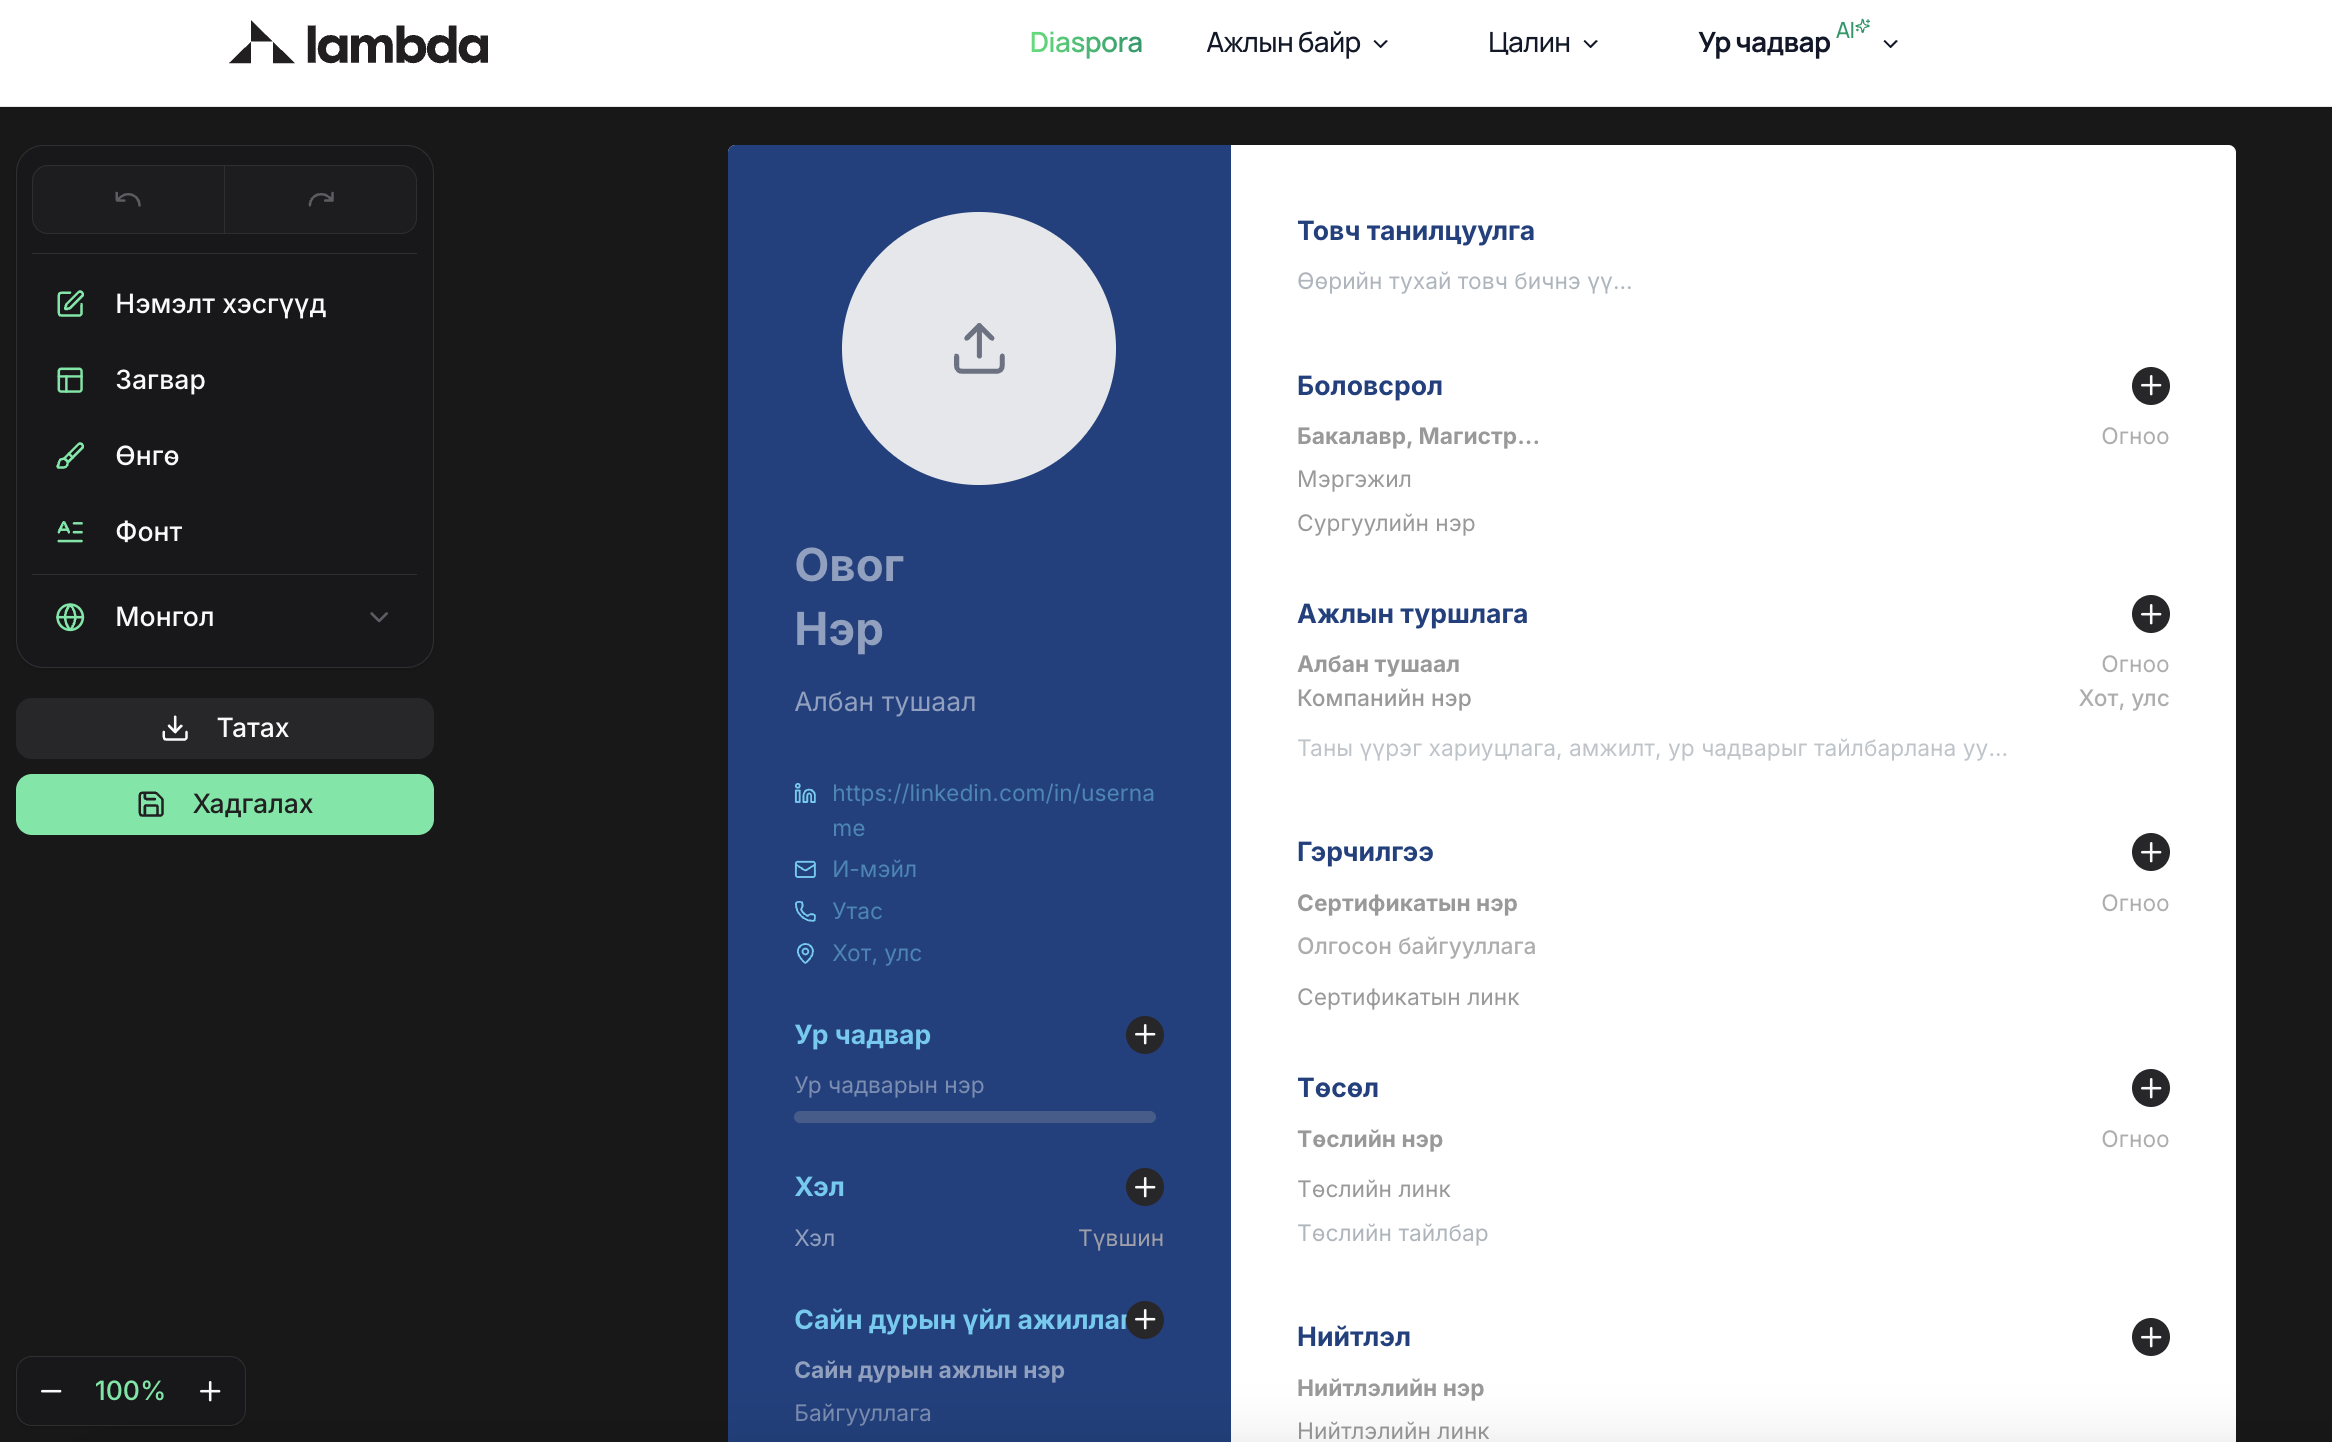
\includegraphics[scale=0.3]{Figures/chapter1/lambda/cv.png}
    \caption{Zangia.mn сайтын анкет үүсгэх хэсэг}
    \label{fig: l-cv}
\end{figure}

\par{}Харьцуулалтын хүснэгтийг доор үзүүлэв.

\label{tab:system_comparison}
\begin{longtable}{| p{5.5cm} | p{2.6cm} | p{3cm} | p{2.8cm} |}
\caption{Судлагдсан системүүдийн харьцуулалт} \\
\hline
{\bfseries Боломж} & {\bfseries Zangia.mn} & {\bfseries Lambda.global} & {\bfseries Хөгжүүлж буй систем} \\ \hline
\endfirsthead
\hline
{\bfseries Боломж} & {\bfseries Zangia.mn} & {\bfseries Lambda.global} & {\bfseries Хөгжүүлж буй систем} \\ \hline
\endhead
{\bf Ажлын зар нийтлэх} & Тийм & Тийм & Тийм \\ \hline
{\bf CV байршуулах} & Тийм & Тийм & Тийм \\ \hline
{\bf AI-д суурилсан CV үнэлгээ} & Тийм & Тийм & Тийм \\ \hline
{\bf Нийцлийн тайлбартай үнэлгээ} & Тийм & Тийм & Тийм \\ \hline
{\bf Ур чадварын даалгавар} & Үгүй & Үгүй & Тийм \\ \hline
{\bf AI чатбот дэмжлэг} & Үгүй & Үгүй & Тийм \\ \hline
{\bf Ярилцлага товлох} & Үгүй & Үгүй & Тийм \\ \hline
\end{longtable}

\par{}Дээрх харьцуулалтаас харахад судлагдсан системүүд нь ажлын зар нийтлэх, CV байршуулах, AI-д суурилсан CV үнэлгээ зэрэг үндсэн боломжуудыг дэмждэг. Гэвч ажил горилогчийн ур чадварыг практик даалгавраар шалгах, AI чатбот ашиглан ажлын мэдээлэл хайх, ярилцлага товлох зэрэг цогц боломжуудыг хангадаггүй байна. Боловсруулж буй систем нь эдгээр дутагдлуудыг нэг платформ дотор шийдвэрлэхэд чиглэгдсэн болно.
\section{Хөгжүүлэлтэд ашиглах алгоритм}

\par{}Энэхүү судалгаанд ажил горилогчийн CV болон ажлын байрны тодорхойлолтын хоорондын нийцлийг тодорхойлох зорилгоор томоохон хэлний загвар (Large Language Model, LLM)-д суурилсан аргыг ашиглана.

\par{}Уламжлалт embedding болон cosine similarity-д суурилсан аргууд нь зөвхөн тоон ижил төстэй байдлыг хэмжиж, яагаад тохирч байгааг тайлбарлах боломж хязгаарлагдмал байдаг. Харин LLM-д суурилсан арга нь CV болон ажлын байрны шаардлагыг контекстын түвшинд ойлгон дүн шинжилгээ хийж, тайлбарлах боломжтой.

\par{}Тодруулбал, Anthropic компанийн Claude Sonnet загварыг ашиглан дараах алхмуудаар үнэлгээ хийнэ:
\begin{enumerate}
    \item CV-ийн текстийг PDF файлаас задлана;
    \item Ажлын байрны гарчиг, шаардлага, ур чадвар, үүрэгт ажилтай хамт prompt бүтээнэ;
    \item Claude API-д prompt илгээж, бүтэцтэй JSON хариулт авна;
    \item JSON хариултад: нийт оноо, тойм, тохирсон ур чадварууд, дутуу ур чадварууд, зөвлөмжүүд орно.
\end{enumerate}

\par{}Энэхүү арга нь дараах давуу талуудтай:
\begin{itemize}
    \item Тайлбарлах боломжтой (explainable) — аль ур чадвар яагаад тохирсон/дутуу байгааг тайлбарладаг;
    \item Тусдаа Python/ML сервер шаардахгүй — Go-оос шууд дуудна;
    \item Context-aware — CV болон ажлын байрны агуулгыг гүн ойлгох боломжтой.
\end{itemize}

\par{}Чатботын хувьд өгөгдлийн санд суурилсан контекст оруулах (context injection) аргыг ашигласан. Систем нь хэрэглэгчийн мессежийг хүлээн авах бүрт PostgreSQL өгөгдлийн сангаас бүх идэвхтэй (\texttt{posted}) ажлын байрны гарчиг, байршил, цалин, ур чадварын мэдээллийг татаж, тэдгээрийг Claude-ийн prompt-д контекст болгон нэмдэг. Ингэснээр чатбот нь хэрэглэгчийн асуултад бодит, тухайн үеийн мэдээлэлд суурилсан хариулт өгнө.

\par{}Иймээс LLM-д суурилсан, өгөгдлийн сангийн мэдээллийг prompt-д шууд дамжуулах арга нь CV-ажлын байрны нийцэл болон чатботын асуудлыг шийдвэрлэхэд тохиромжтой гэж үзэж байна.

%-------------------------------------------------------------------------------

\section{Технологийн судалгаа}
\paragraph{} Системийн back-end болон front-end хөгжүүлэлтэд ашиглах технологиуд болон хөгжүүлэлтийг хэрэгжүүлэхэд шаардлагатай хөгжүүлэлтийн орчны тайлбар судалгаа зэргийг агуулсан.
\subsection*{Back-End хөгжүүлэлтэд ашиглах технологиуд}
\subsubsection*{Go (Golang) программчлалын хэл}
\par
Go буюу Golang нь 2009 онд Google компанийн Роберт Гриземер, Роб Пайк, Кен Томпсон нарын хөгжүүлсэн, нээлттэй эхийн, өндөр гүйцэтгэлтэй программчлалын хэл юм \cite{golang2024}. Go хэл нь сервер талын веб систем, микросервис архитектур, сүлжээний програмчлал зэрэгт өргөн хэрэглэгддэг.

\par Go хэлний онцлог давуу талууд:
\begin{itemize}
    \item \textbf{Өндөр гүйцэтгэл:} C/C++ хэлтэй ойролцоо хурдтай;
    \item \textbf{Concurrency дэмжлэг:} Goroutine болон channel ашиглан олон урсгалт ажиллагааг хялбар хэрэгжүүлдэг;
    \item \textbf{Хялбар синтакс:} Суралцахад хялбар, цэвэр бүтэцтэй;
    \item \textbf{Стандарт сангийн баялаг багц:} HTTP сервер, JSON боловсруулалт, криптограф зэрэг суурь функцууд бэлэн.
\end{itemize}

Энэхүү системд Go хэлийг REST API хөгжүүлэх, хиймэл оюунтай холбогдох логик, анкет үнэлгээний алгоритм, өгөгдлийн сангийн холболт зэрэг үндсэн бизнес логикийг хэрэгжүүлэхэд ашиглана.
\begin{figure}[H]
    \centering
    
\includegraphics[scale=0.1]{Figures/chapter1/golang.png}
    \caption{Golang лого}
    \label{fig: golang logo}
\end{figure}

\subsubsection*{Chi router}
\par
Chi нь Go хэл дээр бичигдсэн HTTP router бөгөөд REST API \cite{fielding2000rest} хөгжүүлэхэд тохиромжтой.

\par Chi router-ийн давуу талууд:
\begin{itemize}
    \item \textbf{Хөнгөн, хурдан ажиллагаа:} Минимал бүтэцтэй тул өндөр гүйцэтгэлтэй;
    \item \textbf{Middleware дэмжлэг:} Request боловсруулалтыг шаталсан байдлаар удирдах боломжтой;
    \item \textbf{REST API-д тохиромжтой:} Endpoint-уудыг цэгцтэй зохион байгуулна.
\end{itemize}

Энэхүү системд Chi router-ийг backend API хөгжүүлэх, frontend болон AI service хооронд мэдээлэл дамжуулахад ашиглана.
\begin{figure}[H]
    \centering
    
\includegraphics[scale=0.2]{Figures/chapter1/go-chi.png}
    \caption{Chi router лого}
    \label{fig: go-chi logo}
\end{figure}

\subsection*{Front-End хөгжүүлэлтэд ашиглах технологиуд}

\subsubsection*{Nuxt.js}
\par
Nuxt.js нь Vue.js дээр суурилсан, сервер болон клиент талын рендерингийг дэмждэг веб framework юм \cite{nuxtjs2024}. Энэ нь орчин үеийн, хурдан ажиллагаатай веб аппликейшн хөгжүүлэхэд өргөн хэрэглэгддэг.

\par Nuxt.js-ийн давуу талууд:
\begin{itemize}
    \item \textbf{SSR болон CSR дэмжлэг:} Сервер болон клиент талын рендерингийг дэмждэг;
    \item \textbf{Component-based архитектур:} Кодыг дахин ашиглах боломжтой;
    \item \textbf{Хөгжүүлэлтийн хялбар орчин:} Routing, state management зэрэг нь автомат зохицуулагддаг.
\end{itemize}

Энэхүү системд Nuxt.js-ийг хэрэглэгчийн интерфэйс хөгжүүлэх, CV болон ажлын байрны мэдээлэл оруулах, үнэлгээний үр дүн харуулах зэрэг үйлдлүүдийг хэрэгжүүлэхэд ашиглана.
\begin{figure}[H]
    \centering
    
\includegraphics[scale=0.2]{Figures/chapter1/nuxtjs.png}
    \caption{Nuxt.js лого}
    \label{fig: nuxtjs logo}
\end{figure}

\subsubsection*{Tailwind CSS}
\par
Tailwind CSS нь utility-first зарчимд суурилсан CSS framework бөгөөд веб интерфэйсийг хурдан, уян хатан байдлаар хөгжүүлэх боломжийг олгодог.

\par Tailwind CSS-ийн давуу талууд:
\begin{itemize}
    \item \textbf{Хурдан хөгжүүлэлт:} Бэлэн utility классууд ашиглан UI хурдан бүтээнэ;
    \item \textbf{Responsive дизайн:} Янз бүрийн төхөөрөмжид тохирсон интерфэйс хийхэд хялбар;
    \item \textbf{Customizable:} Дизайныг өөрийн шаардлагад тохируулан өөрчлөх боломжтой.
\end{itemize}

Энэхүү системд Tailwind CSS-ийг хэрэглэгчийн интерфэйсийн загвар, layout болон responsive дизайн хийхэд ашиглана.
\begin{figure}[H]
    \centering
    
\includegraphics[scale=0.05]{Figures/chapter1/Tailwind_CSS.png}
    \caption{Tailwind CSS лого}
    \label{fig: tailwind logo}
\end{figure}
\subsubsection*{shadcn/vue компонентын сан}
\par
shadcn/vue нь Vue.js дээр суурилсан UI компонентын сан бөгөөд орчин үеийн, цэвэр дизайнтай интерфэйс бүтээхэд ашиглагддаг.

\par shadcn/vue-ийн давуу талууд:
\begin{itemize}
    \item \textbf{Бэлэн компонентууд:} Button, form, dialog зэрэг UI элементүүд бэлэн;
    \item \textbf{Орчин үеийн дизайн:} Хэрэглэгчид ээлтэй, минимал хэв маягтай;
    \item \textbf{Tailwind-тэй уялдаа:} Tailwind CSS-тэй хамт ашиглахад тохиромжтой.
\end{itemize}

Энэхүү системд shadcn/vue-ийг форм, товч, popup зэрэг интерфэйсийн элементүүдийг бүтээхэд ашиглана.
\begin{figure}[H]
    \centering
    
\includegraphics[scale=0.2]{Figures/chapter1/shadcn.jpg}
    \caption{Shadcn ui лого}
    \label{fig: shadcn logo}
\end{figure}
\subsection*{AI service}
\subsubsection*{Anthropic Claude API}
\par
Anthropic Claude API нь томоохон хэлний загвар (LLM)-д суурилсан хиймэл оюуны үйлчилгээ бөгөөд байгалийн хэл боловсруулалт, текст дүн шинжилгээ, асуулт-хариулт зэрэг олон зорилгоор ашиглагддаг.

\par Claude API-ийн давуу талууд:
\begin{itemize}
    \item \textbf{Тусдаа AI сервер шаардахгүй:} Go backend-ээс шууд REST API дуудлагаар ашиглана;
    \item \textbf{Explainable гаралт:} Бүтэцтэй JSON хэлбэрээр тайлбартай үнэлгээ буцаана;
    \item \textbf{Контекст оруулахад тохиромжтой:} Өгөгдлийн сангаас олж авсан мэдээллийг prompt-д шууд нэмж, нарийвчлалтай хариулт үүсгэх боломжтой;
    \item \textbf{Зардал:} Claude Sonnet загвар нь нэг үнэлгээнд ойролцоогоор \$0.02 зарцуулна.
\end{itemize}

Энэхүү системд Claude API-г CV үнэлгээ, чатботын хариулт үүсгэх болон даалгавар автоматаар үүсгэхэд ашиглана.
\subsection*{Өгөгдлийн сан}

\subsubsection*{PostgreSQL өгөгдлийн сан}
\par
PostgreSQL нь нээлттэй эхтэй, найдвартай, өргөтгөх боломжтой харилцаат өгөгдлийн сангийн систем юм \cite{postgresql2024}.

\par PostgreSQL-ийн давуу талууд:
\begin{itemize}
    \item \textbf{Найдвартай байдал:} ACID шинж чанарыг бүрэн дэмждэг;
    \item \textbf{Өгөгдлийн уян хатан байдал:} JSON болон бүтэцтэй өгөгдлийг хадгалах боломжтой;
    \item \textbf{Өргөтгөх боломж:} Том хэмжээний системд ашиглах боломжтой.
\end{itemize}

Энэхүү системд PostgreSQL-ийг хэрэглэгч, CV, ажлын байр, үнэлгээний үр дүн зэрэг өгөгдлийг хадгалахад ашиглана.
\begin{figure}[H]
    \centering
    
\includegraphics[scale=0.2]{Figures/chapter1/postgres.png}
    \caption{PostgreSQL лого}
    \label{fig: postgres logo}
\end{figure}

\subsection*{Хөгжүүлэлтийн орчин}
\subsubsection*{Visual Studio Code IDE}
\par
Visual Studio Code нь Microsoft компанийн хөгжүүлсэн хөнгөн жинтэй код засварлагч юм. Go, JavaScript, Vue, Tailwind CSS, SQL зэрэг олон хэл дэмждэг бөгөөд өргөтгөлүүдээр дамжуулан Git, Docker, Postgres зэрэгтэй шууд ажиллах боломжтой.

\begin{figure}[H]
    \centering
    
\includegraphics[scale=0.05]{Figures/chapter1/vscode.png}
    \caption{ Visual Studio Code лого}
    \label{fig: vscode logo}
\end{figure}
\subsection*{Кодын менежмент}
%Кодын менежментийг хэрхэн гүйцэтгэсэн, кодыг хаана байршуулж хөгжүүлсэн талаар бичнэ. GitHub, Gitlab etc.

\par{}Энэхүү системийн хөгжүүлэлтэд кодын менежментийг Git хувилбарын удирдлагын систем болон GitHub платформыг ашиглан хэрэгжүүлнэ. Git нь кодын өөрчлөлтийг хянах, хөгжүүлэлтийн явцыг удирдах, өмнөх хувилбарууд руу буцах боломжийг олгодог.

\par{}Git-ийн давуу талууд:
\begin{itemize}
    \item \textbf{Өөрчлөлтийн хувилбауудын хяналт:} Кодын өөрчлөлтийн түүхийг хадгална;
    \item \textbf{Branch ашиглах:} Шинэ боломжуудыг тусгаарлан хөгжүүлэх боломжтой;
    \item \textbf{Аюулгүй байдал:} Кодыг алдах эрсдлийг бууруулна.
\end{itemize}

\par{}GitHub нь Git-д суурилсан онлайн repository үйлчилгээ бөгөөд код хадгалах, нөөцлөх, хамтран хөгжүүлэх боломжийг бүрдүүлдэг.

\par{}GitHub-ийн давуу талууд:
\begin{itemize}
    \item \textbf{Remote repository:} Кодыг онлайн хадгалах боломж;
    \item \textbf{Pull request:} Кодын өөрчлөлтийг шалгах, нэгтгэх;
    \item \textbf{Issue tracking:} Алдаа болон шинэ боломжуудыг удирдах.
\end{itemize}

\par{}Энэхүү төсөлд GitHub ашиглан кодын санг хадгалж, хөгжүүлэлтийн явцыг удирдах, өөрчлөлтийн түүхийг хянах байдлаар ашиглана.


\section*{Бүлгийн дүгнэлт}
%-------------------------------------------------------------------------------
\par{}Энэхүү бүлэгт ажил горилогчийн ур чадварыг үнэлэх системийг хөгжүүлэхэд шаардлагатай онол, арга зүйн судалгааг хийсэн. Эхлээд ажилд авах үйл явцыг тодорхойлж, уламжлалт аргын сул талуудыг тодруулан, AI-д суурилсан ажилд авах системүүдийн давуу болон сул талуудыг харьцуулан судалсан.

\par{}AI-д суурилсан үнэлгээний алгоритмуудын судалгааны хүрээнд машин сургалт, байгалийн хэл боловсруулалт (NER, SVM, KNN), гүн сургалтын embedding аргууд (Sentence-BERT, Siamese network) болон томоохон хэлний загвар (LLM)-уудыг авч үзсэн. Судалгааны үр дүнд уламжлалт алгоритмуудын "black-box" шинж чанар болон тайлбарлах хүндрэлийг харгалзан, тайлбарлах боломжтой (explainable) үнэлгээ гаргах чадвартай LLM-д суурилсан аргыг сонгон авсан.

\par{}Ижил төстэй системүүдийн судалгааны хүрээнд Монголын зах зээлд үйл ажиллагаа явуулдаг zangia.mn болон lambda.global системүүдийн онцлог, давуу болон сул талуудыг судалж, харьцуулалтын хүснэгтийг гаргасан. Судалгааны дүнгээс одоогийн системүүд нь ажлын зар, CV байршуулах, AI CV үнэлгээ зэрэг үндсэн боломжуудыг дэмждэг ч ур чадварын практик даалгавар, AI чатбот болон ярилцлага товлох функцийг агуулдаггүй нь тодорхой болсон.

\par{}Хөгжүүлэлтэд ашиглах алгоритм болон технологиудыг тодорхойлох хүрээнд CV болон ажлын байрны нийцлийг LLM (Anthropic Claude Sonnet)-ээр тайлбарлан үнэлэх арга, чатботод PostgreSQL-д суурилсан контекст оруулах арга зүйг сонгосон. Back-end хэсэгт Go болон Chi router, front-end хэсэгт Nuxt.js, Tailwind CSS, shadcn/vue, өгөгдлийн санд PostgreSQL, хувилбарын удирдлагад Git болон GitHub технологиудыг хөгжүүлэлтэд ашиглахаар тодорхойлсон. Дараагийн бүлэгт дурдсан судалгаанд тулгуурлан системийн шаардлага болон шинжилгээг авч үзнэ.